\documentclass{article}
\usepackage{amsmath}
\usepackage{amsfonts}
\usepackage{amssymb}
\usepackage{amsthm}
\usepackage{bm}
\usepackage{graphicx}
\usepackage[makeroom]{cancel}

\begin{document}
\section{Problem 1}
\subsection{Mathematical Analysis}
Let's consider this generic formula, to classify new vector $\textbf{x}$:\\
$\displaystyle\arg\max_{c\in\mathcal{C}}\frac{p(y=c)p(\textbf{x}|y=c)}{\displaystyle\sum_{c\in \mathcal{C}}p(y=c)p(\textbf{x}|y=c) }$.
In our case the class conditional probabilities are modelled as normal distributions so this means, using the notation from \cite{Murphy} 
that the above formula translates in:\\
$\displaystyle\arg\max_{c\in\mathcal{C}}\frac{\pi_c|2\pi\bm{\Sigma}_c|^{-\frac{1}{2}}\textbf{exp}[-\frac{1}{2}(\textbf{x}-\bm{\mu}_c)^{T}\bm{\Sigma}^{-1}_c(\textbf{x}-\bm{\mu}_c)]}{\displaystyle\sum_{c\in\mathcal{C}}\pi_c|2\pi\bm{\Sigma}_c|^{-\frac{1}{2}}\textbf{exp}[-\frac{1}{2}(\textbf{x}-\bm{\mu}_c)^{T}\bm{\Sigma}^{-1}_c(\textbf{x}-\bm{\mu}_c)]}$. Where $\pi_c$ are the prior probabilities, $\bm{\mu}_c$ the means and $\bm{\Sigma}_c$ the covariance matrices for every class. Notice that performing the previous maximization is the same (by the property of the exponential) as minimizing
the following formula: $(\textbf{x}-\bm{\mu}_c)^{T}\bm{\Sigma}^{-1}_c(\textbf{x}-\bm{\mu}_c)$ which is called Mahalanobis distance and 
which is indeed what we implemented in our code because we wanted to be able to call a single function from both QDAlearn and LDAlearn functions, and 
hence we needed to be general.
But to see why we get linear and quadratic boundaries let's keep analyzing the exponenential formula.
In LDA we make the assumption that:  $\forall\ c\in\mathcal{C}\ \bm{\Sigma}_c=\bm{\Sigma}$ so we can rewrite the above formula as:\\
$\displaystyle\arg\max_{c\in\mathcal{C}}\frac{\pi_c\textbf{exp}[-\frac{1}{2}(\textbf{x}-\bm{\mu}_c)^{T}\bm{\Sigma}^{-1}(\textbf{x}-\bm{\mu}_c)]}{\displaystyle\sum_{c\in\mathcal{C}}\pi_c\textbf{exp}[-\frac{1}{2}(\textbf{x}-\bm{\mu}_c)^{T}\bm{\Sigma}^{-1}(\textbf{x}-\bm{\mu}_c)]}$.
With some calculations we can go further and see the equality with:
\begin{align}
\displaystyle\arg\max_{c\in\mathcal{C}}\frac{\textbf{exp}[log(\pi_c)+\bm{\mu}_c^T\bm{\Sigma}^{-1}\textbf{x}-\frac{1}{2}\textbf{x}^T\bm{\Sigma}^{-1}\textbf{x}-\frac{1}{2}\bm{\mu}_c\bm{\Sigma}^{-1}\bm{\mu}_c]}{\displaystyle\sum_{c\in \mathcal{C}}\textbf{exp}[log(\pi_c)+\bm{\mu}_c^T\bm{\Sigma}^{-1}\textbf{x}-\frac{1}{2}\textbf{x}^T\bm{\Sigma}^{-1}\textbf{x}-\frac{1}{2}\bm{\mu}_c\bm{\Sigma}^{-1}\bm{\mu}_c]}=\\
\displaystyle\arg\max_{c\in\mathcal{C}}\frac{\cancel{\textbf{exp}[-\frac{1}{2}\textbf{x}^T\bm{\Sigma}^{-1}\textbf{x}]}\cdot\textbf{exp}[log(\pi_c)+\bm{\mu}_c^T\bm{\Sigma}^{-1}\textbf{x}-\frac{1}{2}\bm{\mu}^T_c\bm{\Sigma}^{-1}\bm{\mu}_c]}{\cancel{\textbf{exp}[-\frac{1}{2}\textbf{x}^T\bm{\Sigma}^{-1}\textbf{x}]}\cdot\displaystyle\sum_{c\in \mathcal{C}}\textbf{exp}[log(\pi_c)+\bm{\mu}_c^T\bm{\Sigma}^{-1}\textbf{x}-\frac{1}{2}\bm{\mu}_c\bm{\Sigma}^{-1}\bm{\mu}_c]}.
\end{align}
So we can see that the only quadratic term in $\textbf{x}$ got cancelled out. Since we only care about the maximum class probability we can disregard about the denominator (which doesn't vary with $\textbf{c}$) and consider only:\\
$\displaystyle\arg\max_{c\in\mathcal{C}}\textbf{exp}[log(\pi_c)+\bm{\mu}_c^T\bm{\Sigma}^{-1}\textbf{x}-\frac{1}{2}\bm{\mu}^T_c\bm{\Sigma}^{-1}\bm{\mu}_c]$. Since log is a monotonic function we can disregard the exponentiation and only care about what is inside it, getting:
$\displaystyle\arg\max_{c\in\mathcal{C}}\ log(\pi_c)+\bm{\mu}_c^T\bm{\Sigma}^{-1}\textbf{x}-\frac{1}{2}\bm{\mu}^T_c\bm{\Sigma}^{-1}\bm{\mu}_c$.\\
In our case the prior probabilities  $\pi_c$ for every class where all very similar and about $20\%$ so we can disregard them, and consider only:\\
$\displaystyle\arg\max_{c\in\mathcal{C}}\bm{\mu}_c^T\bm{\Sigma}^{-1}\textbf{x}-\frac{1}{2}\bm{\mu}^T_c\bm{\Sigma}^{-1}\bm{\mu}_c$.
The previous formula is \textbf{linear} in $\textbf{x}$ and indeed if we consider the boundary with any two classes $c,c'\in\mathcal{C}$ given by the equation:
$p(y=c^{'}|\textbf{x})=p(y=c|\textbf{x})$ iff $\bm{\mu}_{c'}^T\bm{\Sigma}^{-1}\textbf{x}-\frac{1}{2}\bm{\mu}^T_{c'}\bm{\Sigma}^{-1}\bm{\mu}_{c'}=
\bm{\mu}_c^T\bm{\Sigma}^{-1}\textbf{x}-\frac{1}{2}\bm{\mu}^T_c\bm{\Sigma}^{-1}\bm{\mu}_c$ we see that this is the equation of a line.
In the case of QDA we cannot perform the canceling from (1) to (2) and so we end up with a quadratic term in $\textbf{x}$ in the final equation 
and this is why we end up with quadratic boundaries.
\subsection{Experimental Results}
The accuracy achieved with LDA is $97\%$ while with QDA is $94\%$: evidently the data is best separated by lines and not by curves.
In the following we can see the graphic results of LDA and QDA:
\begin{figure}[h]
  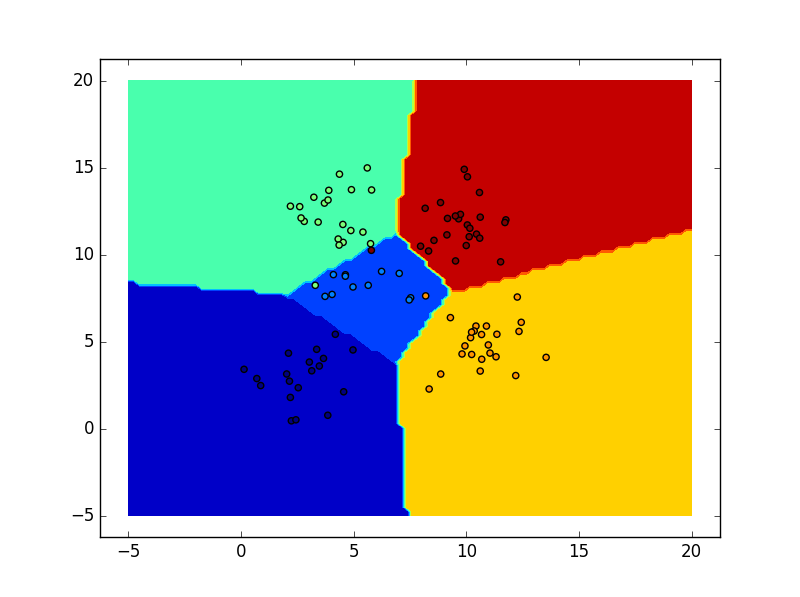
\includegraphics[width=\textwidth]{lda.png}
  \caption{LDA}
\end{figure}
\begin{figure}[h]
  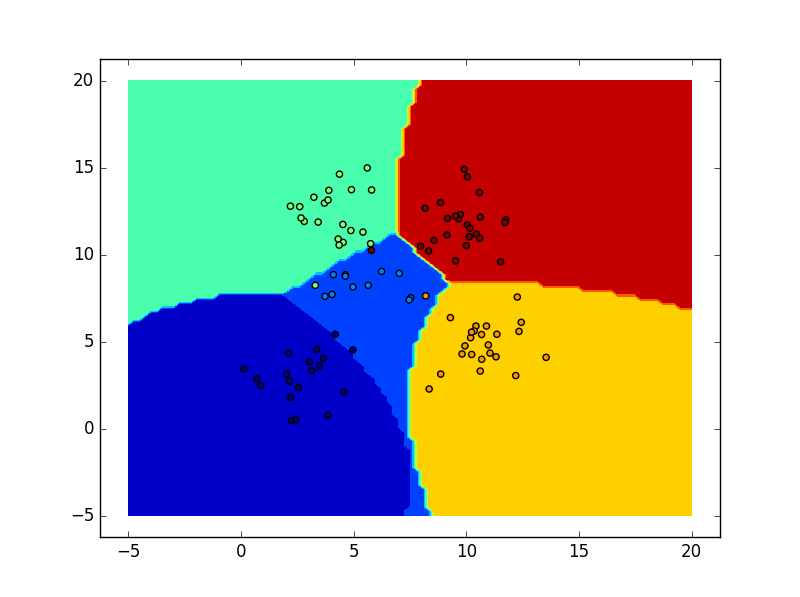
\includegraphics[width=\textwidth]{qda.png}
  \caption{QDA}
\end{figure}
\bibliographystyle{unsrt}
\bibliography{bib}
\end{document}